\documentclass[10pt]{article}
\usepackage[utf8]{inputenc}
\usepackage{amsmath}
\usepackage{amsfonts}
\usepackage{tikz}
\usepackage{amssymb}
%\usepackage{fullpage}
\usepackage[top=1in, bottom=1in, left=1in, right=1in]{geometry}
\usepackage{graphicx}
\usepackage{hyperref}
\usepackage{subcaption}
\usepackage{float}
\usepackage[section]{placeins}
\graphicspath{{./FigJar/}}
\begin{document}
\author{Erdem M. Karaköylü}
\title{A Principled Approach to Developing Chlorophyll Models for Remote Sensing}
\date{\today}
\maketitle
\tableofcontents
\newpage

\newcommand{\reddash}{\raisebox{2pt}{\tikz{\draw[-,red,dashed,line width=1.2pt](0,0) -- (5mm,0);}}}
\newcommand{\blkdash}{\raisebox{2pt}{\tikz{\draw[-,black,dashed,line width=1.2pt](0,0) -- (5mm,0);}}}
\newcommand{\blksold}{\raisebox{2pt}{\tikz{\draw[-,black,solid,line width=1.2pt](0,0) -- (5mm,0);}}}
\section{Abstract}

\newpage

\section{Introduction}
	\subsection{Background}
		\begin{itemize}
		\item Necessity for estimating chlorophyll
		\item Opportunities afforded by chlorophyll estimation through remote sensing
		\item State of current chlorophyll algorithms for remote sensing
		\begin{itemize}
		    \item OC4 for SeaWiFS$\rightarrow$there is a dichotomy in remote sensing between empirical models and quasi-analytical models. Empirical models are so-called because their structure is dictated by their ability to fit the training data, often without any inter-model comparison, or post-training model skill assessment exercise. As a result, these are high order polynomials that are emminently uninterpretable with regards to the predictor data used. Moreover because of the training method used, they are overfitting the training data used and are therefor rarely generalizable to the variety of regions sampled remotely. Quasi analytical models (QAA), on the other hand claim an origin in first principles but end up resorting to some degree of empiricism as described above, where first principles fall short. In short, empirical models are frowned upon because they are inscrutable and don't work well for anything but the open ocean; QAAs are frowned upon because they don't work well. The contention of the present paper is that such a dichotomy is unnecessary.
		    \item Hu \& Franz 2012
		    \item Gholizadeh et al (2015?)
		\end{itemize}
		\item Basic empirical form
		\begin{align}
		log_{10}\left(chlor_a\right) = a_0 + \sum_{i=1}^ja_ilog_{10}\left(\frac{max\left(Rrs	\left(\lambda_{blue}\right)\right)}{Rrs\left(\lambda_{green}\right)}\right)
		\end{align}
		\item Problems with current algorithms:
		\begin{itemize}
			\item collinearity of inputs
			\item poor performance in coastal
			\item maximum likelihood estimation approach $\rightarrow$ risk of overfitting (lack of in-situ data vailability  compared to satellite data makes it worse)
		\end{itemize}
	\end{itemize}
	
	\subsection{Proposed framework}
	    Here, I use  Bayesian regression models to predict chlorophyll concentration from apparent optical properties. There are a number of advantages for adopting this approach. The first of these is a problem agnostic set of steps detailed in the methods section. A second advantage is that model construction is transparent and assumptions are laid bare. This makes any model developed with this framework easily, and constructively, criticizable. A positive spillover of this is that the process requires that the model code be made available for model criticism to occur; i.e. the study in question must be reproducible to be effective. Another attractive feature of the Bayesian framework is that rather than point predictions, the output of the Bayesian model is the posterior distribution. The posterior distibution is a rich construct that can be used to develop insight in the process of interest, uncertainties around predictions, and a means to rank model performance. Finally, Bayesian regression models are inherently regularized through the stipulated priors. This has a 'calming' effect on the model, which is less likely to overfit an inappropriately scant data set; a common problem in bio-optical model development for marine remote sensing. 


Succintly, this approach ensures:
	\begin{itemize}
		\item transparent construction of models with explicit formulation of assumptions,
		\item assumptions/background information codified as priors that are easy to criticize and modify;
		\item verifiable prior feasibility before data collection via prior predictive checks
		\item built-in regularization, which lessens the risk of overfitting;
		\item built-in structure for selecting relevant features;
		\item posterior distribution as rich information structure from which to estimate parameter uncertainty, output predictin uncertainty, and likelihood of model performance on out-of-sample data;
		\item assessment of predictive ability via posterior predictive checks;
		\item multiple model development, which avoids overemphasis on any particular formulation;
		\item evaluation/comparison between models using information theory.
	\end{itemize}

For the sake of reproducibility of the models and their results, the code for both data preparation, model construction and fitting and result assessment are available from the github repository [here]. In addition,  the data in their various stages of processing (raw, standardized, split, transformed), are available from the Open Science Framework (OSF) page associated with this projet, [here].
			
\newpage			
%----------------- END INTRODUCTION --------------------------

\section{Methods}
	\subsection{Model Development}
	Four models are developed here		
		\subsubsection{Bayesian Linear Regression}
			\begin{itemize}
				\item Order 1 regression for interpretable coefficients
				\item no interaction terms
				\item regularized horseshoe prior for feature selection
			\end{itemize}
		\subsubsection{Bayesian Linear Regression with Interaction Terms}
			\begin{itemize}
				\item generation of 1st order interaction terms
				\item allowing for both strong and weak heredity
			\end{itemize}
		\subsubsection{Bayesian Neural Network}
			\begin{itemize}
				\item Specific hierarchical structure for ARD
				\item HL1 4 NN with elu activation
			\end{itemize}
		\subsubsection{Bayesian OC4 version as Baseline}
	
	\subsection{Prior Predictive Checks}
	
	\subsection{Data Acquisition/Exploration/Transformation}
	    \subsubsection{Data exploration and transformation}
	        \begin{itemize}
	            \item
	        \end{itemize}
		\subsubsection{Basis reduction via PCA}
		    \begin{itemize}
			    \item PCA of Rrs to reduce overlap of information between predictor variables
		    \end{itemize}
	
	\subsection{Model Fitting}
	
	\subsection{Marginal Posterior of Coefficients $\rightarrow$ Feature Relevance Determination}	
	
	\subsection{Posterior Predictive Checks}
	
	\subsection{Model Comparison Through Posterior Predictive Checks}
	
%----------------- END METHODS --------------------------

\section{Results}

%----------------- END RESULTS --------------------------


%----------------- END DISCUSSION --------------------------


	
\end{document}
			
		%	\begin{figure}[H]
		%		\centering
		%		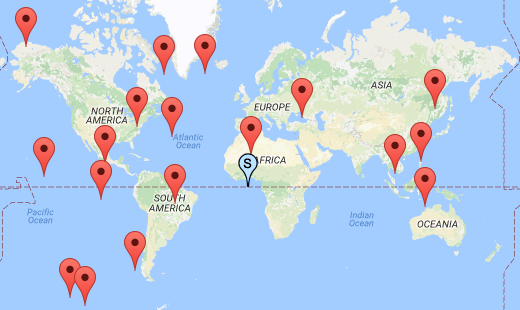
\includegraphics[scale=0.5]{randomMapPts.png}
		%		\caption{Random sampling of 18 geographic locations}
		%	\end{figure}
		